\problemname{Mineralų telkiniai}

\illustration{.3}{img/turnbull.jpg}{Eroding mud face exposing new minerals. Photo: Michael D.\ Turnbull, licence: CC BY-SA.}

\noindent
Dirbate nežemiškų iškasenų kompanijoje ir joje užsiimate signalų apdorojimu. 
Šiuo metu jūsų kosminis laivas artėja prie asteroido.
Preliminarūs paviršiaus skenavimas rodo, kad asteroide yra $k$~mineralų telkinių, tačiau jų tikslios vietos nėra žinomos.

\medskip

Asteroido paviršių galima pavaizduoti koordinačių sistema.
Kiekvieno mineralų telkinio \textit{apytikslė} vieta nusakoma sveikosiomis koordinatėmis:
$i$-ojo telkinio koordinatės yra $(x_i, y_i)$, kur
$-b \le x_i \le b$ ir $-b\le y_i \le b$. %constraint:depositcoords
Čia sveikasis skaičius $b$ yra pradinio skenavimo plotis.

Norėdami nustatyti tikslias mineralų telkinių vietas, galite siųsti zondus į asteroido paviršių.
Zondai siunčiami grupėmis.

Tarkime, norite išsiųsti $d$~zondų grupę į paviršiaus taškus, kurių koordinatės $(s_j,t_j)$ kur $1\leq j\leq d$.
Kai zondas nusileidžia nurodytame taške, 
jis apskaičiuoja Manhatano atstumą iki kiekvieno iš $k$~mineralų telkinių
ir nusiunčia apskaičiuotus atstumus atgal į kosminį laivą.
Visi duomenų paketai laivą pasiekia tuo pačiu metu, todėl neįmanoma nustatyti, kuris zondas kuriuos atstumus atsiuntė.
Taigi zondų grupė apskaičiuoja ir grąžina $k\cdot d$ sveikųjų skaičių, žyminčių atstumus
\[|x_i-s_j| + |y_i - t_j| \qquad\text{visiems } i \in \{1,\ldots,k\} \text{ ir } j \in\{ 1,\ldots,d\}\,.\]

Norite išsiųsti kuo mažiau zondų grupių.


\section*{Sąveika}

Ši užduotis interaktyvi.
Sąveikos pradžioje vienoje eilutėje pateikiami trys sveikieji skaičiai $b$, $k$ ir $w$:
koordinačių sistemos riba~$b$,
mineralų telkinių skaičius~$k$,
ir skaičius~$w$ -- kiek daugiausiai zondų grupių galite siųsti.

Tuomet galite pateikti $w$ užklausų. Kiekviena jų atitinka vieną grupę.
Užklausą sudaro simbolis \texttt{?}, po kurio pateikiama $2d$ tarpais atskirtų sveikųjų skaičių.
Taigi užklausos formatas toks: ,,\texttt{?} $s_1$ $t_1$ $\cdots$ $s_d$ $t_d$``, kur zondų skaičiui~$d$ turi galioti
$1\leq d\leq 2000$. % constraint:wavesize
Reikšmės $(s_i,t_i)$ nurodo $i$-ojo zondo koordinates ir joms turi galioti
$-10^8 \leq s_i \leq 10^8$ bei $-10^8 \leq t_i \leq 10^8$. % constraint:probecoordinates
Atsakymas į užklausą yra viena eilutė, kurioje pateikta $k \cdot d$ sveikųjų skaičių, išrikiuotų nemažėjimo tvarka -- 
Manhatano atstumai tarp kiekvienos poros mineralų telkinio ir zondo vietos.

Bendras siunčiamų zondų skaičius, sudėjus visas grupes, negali viršyti
$2\cdot 10^4.$ % constraint:totalprobes

Sąveika baigiama, kai išvedate eilutę, sudarytą iš simbolio \texttt{!} ir
$k$ tarpais atskirtų taškų $x_1, y_1, x_2, y_2, \ldots x_k, y_k$.
Tai turi būti paskutinė jūsų programos išvesties eilutė.

Sprendimas laikomas teisingu, jei išvedate visų mineralų telkinių vietas. 
Jas galite pateikti bet kuria tvarka.

\section*{Ribojimai ir vertinimas}
Visada galios
$1\leq b \leq 10^8$, % constraint:b
$1 \leq k \leq 20$, % constraint:k
ir
$2 \le w \le 10^4$. % constraint:w

Jūsų sprendimas bus testuojamas su keliomis testų grupėmis, kurių kiekviena verta tam tikro skaičiaus taškų.
Kiekviena testų grupė sudaryta iš įvairių testų.
Testų grupės taškai skiriami tik išsprendus visus grupės testus.
Skiriamas taškų skaičius lygus daugiausiai surinkusio sprendimo taškų skaičiui.

\medskip
\begin{tabular}{lll}
	Grupė & Taškai & Papildomi ribojimai \\\hline
  $1$ & $16$ & $k = 1, w = 10^4$\\
  $2$ & $19$ & $w \ge 500$\\
  $3$ & $11$ & $w \ge 210$\\
  $4$ & $13$ & $w \ge 130$\\
  $5$ & $14$ & $w \ge 3$, $b \le 10^4$\\
  $6$ & $14$ & $w \ge 3$, $b \le 10^7$\\
  $7$ & $13$ & \emph{nėra}
\end{tabular}
\section*{Pavyzdys}
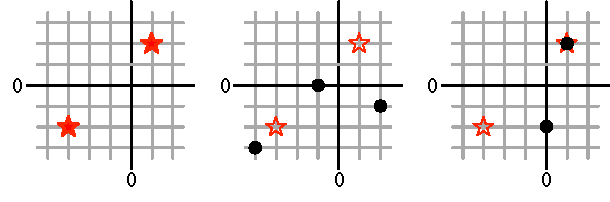
\includegraphics[width=.6\textwidth]{img/sample1.pdf}

Šiame pavyzdyje yra $k=2$ mineralų telkiniai koordinatėse $(1,2)$ ir $(-3,-2)$. Telkiniai pažymėti raudonomis žvaigždutėmis.
Kaip pirmą grupę galėtumėte siųsti $d=3$ zondus į koordinates $(-4,-3)$, $(-1, 0)$ ir $(2,-1)$, pažymėtas juodais taškais.
Ši grupė pateiktų $6$ atstumus: \[
2, 4, 4, 4, 6, 10\,.
\]
Kaip kitą grupę, galėtumėte siųsti $d=2$ zondų į koordinates $(1,2)$ ir $(0,-2)$.
Ši grupė grąžintų $4$ atstumus: \[
0, 3, 5, 8\,.
\]
